\documentclass[aspectratio=169,12pt]{beamer}

\usetheme{Madrid}
\usecolortheme{default}


\usepackage{ctex}

\usepackage{amsmath,amssymb}
\usepackage{graphicx}
\usepackage{booktabs}

\usepackage{hyperref}
\setbeamertemplate{navigation symbols}{}
\setbeamertemplate{footline}{%
  \leavevmode%
  \hbox{%
    \begin{beamercolorbox}[wd=.6\paperwidth,ht=2.5ex,dp=1ex,left]{author in head/foot}%
      \hspace*{2ex}\tiny\textcolor{gray}{Generated by \textbf{ScholarFlow} | GitHub: github.com/bcefghj/scholarflow | 小红书: bcefghj}%
    \end{beamercolorbox}%
    \begin{beamercolorbox}[wd=.4\paperwidth,ht=2.5ex,dp=1ex,right]{date in head/foot}%
      \tiny\insertframenumber{}/\inserttotalframenumber\hspace*{2ex}%
    \end{beamercolorbox}%
  }%
  \vskip0pt%
}

\title{Attention Is All You Need}
\author{Attention Is All You Need}
\date{2024}


\begin{document}

\begin{frame}
\titlepage
\end{frame}


\begin{frame}{Attention Is All You Need}


\begin{itemize}

    \item Ashish Vaswani, Noam Shazeer, Niki Parmar, Jakob Uszkoreit等

    \item Google Brain \& Google Research

    \item 31st Conference on Neural Information Processing Systems (NIPS 2017)

    \item arXiv:1706.03762

\end{itemize}


\end{frame}


\begin{frame}{研究背景与动机}


\begin{itemize}

    \item RNN、LSTM、GRU是序列建模和 transduction 任务的主流方法

    \item RNN的顺序计算特性限制了并行化，在长序列上内存约束明显

    \item 现有模型通过注意力机制连接encoder和decoder

    \item 核心问题：能否用纯注意力机制替代RNN/卷积？

\end{itemize}


\end{frame}


\begin{frame}{相关工作}


\begin{itemize}

    \item Neural GPU、ByteNet、ConvS2S使用卷积作为基本构建块

    \item 卷积模型中两位置间操作数随距离线性或对数增长

    \item Self-attention已在阅读理解、摘要、文本蕴含等任务中成功应用

    \item 本文首次完全基于self-attention实现序列 transduction 模型

\end{itemize}


\end{frame}


\begin{frame}{Transformer模型架构}

\begin{columns}[T]
\begin{column}{0.55\textwidth}

\begin{itemize}

    \item 采用标准的Encoder-Decoder结构

    \item Encoder：将输入序列(x1,...,xn)映射为连续表示z=(z1,...,zn)

    \item Decoder：自回归生成输出序列(y1,...,ym)

    \item 完全基于堆叠的self-attention和逐位置全连接层

\end{itemize}

\end{column}
\begin{column}{0.42\textwidth}
\centering
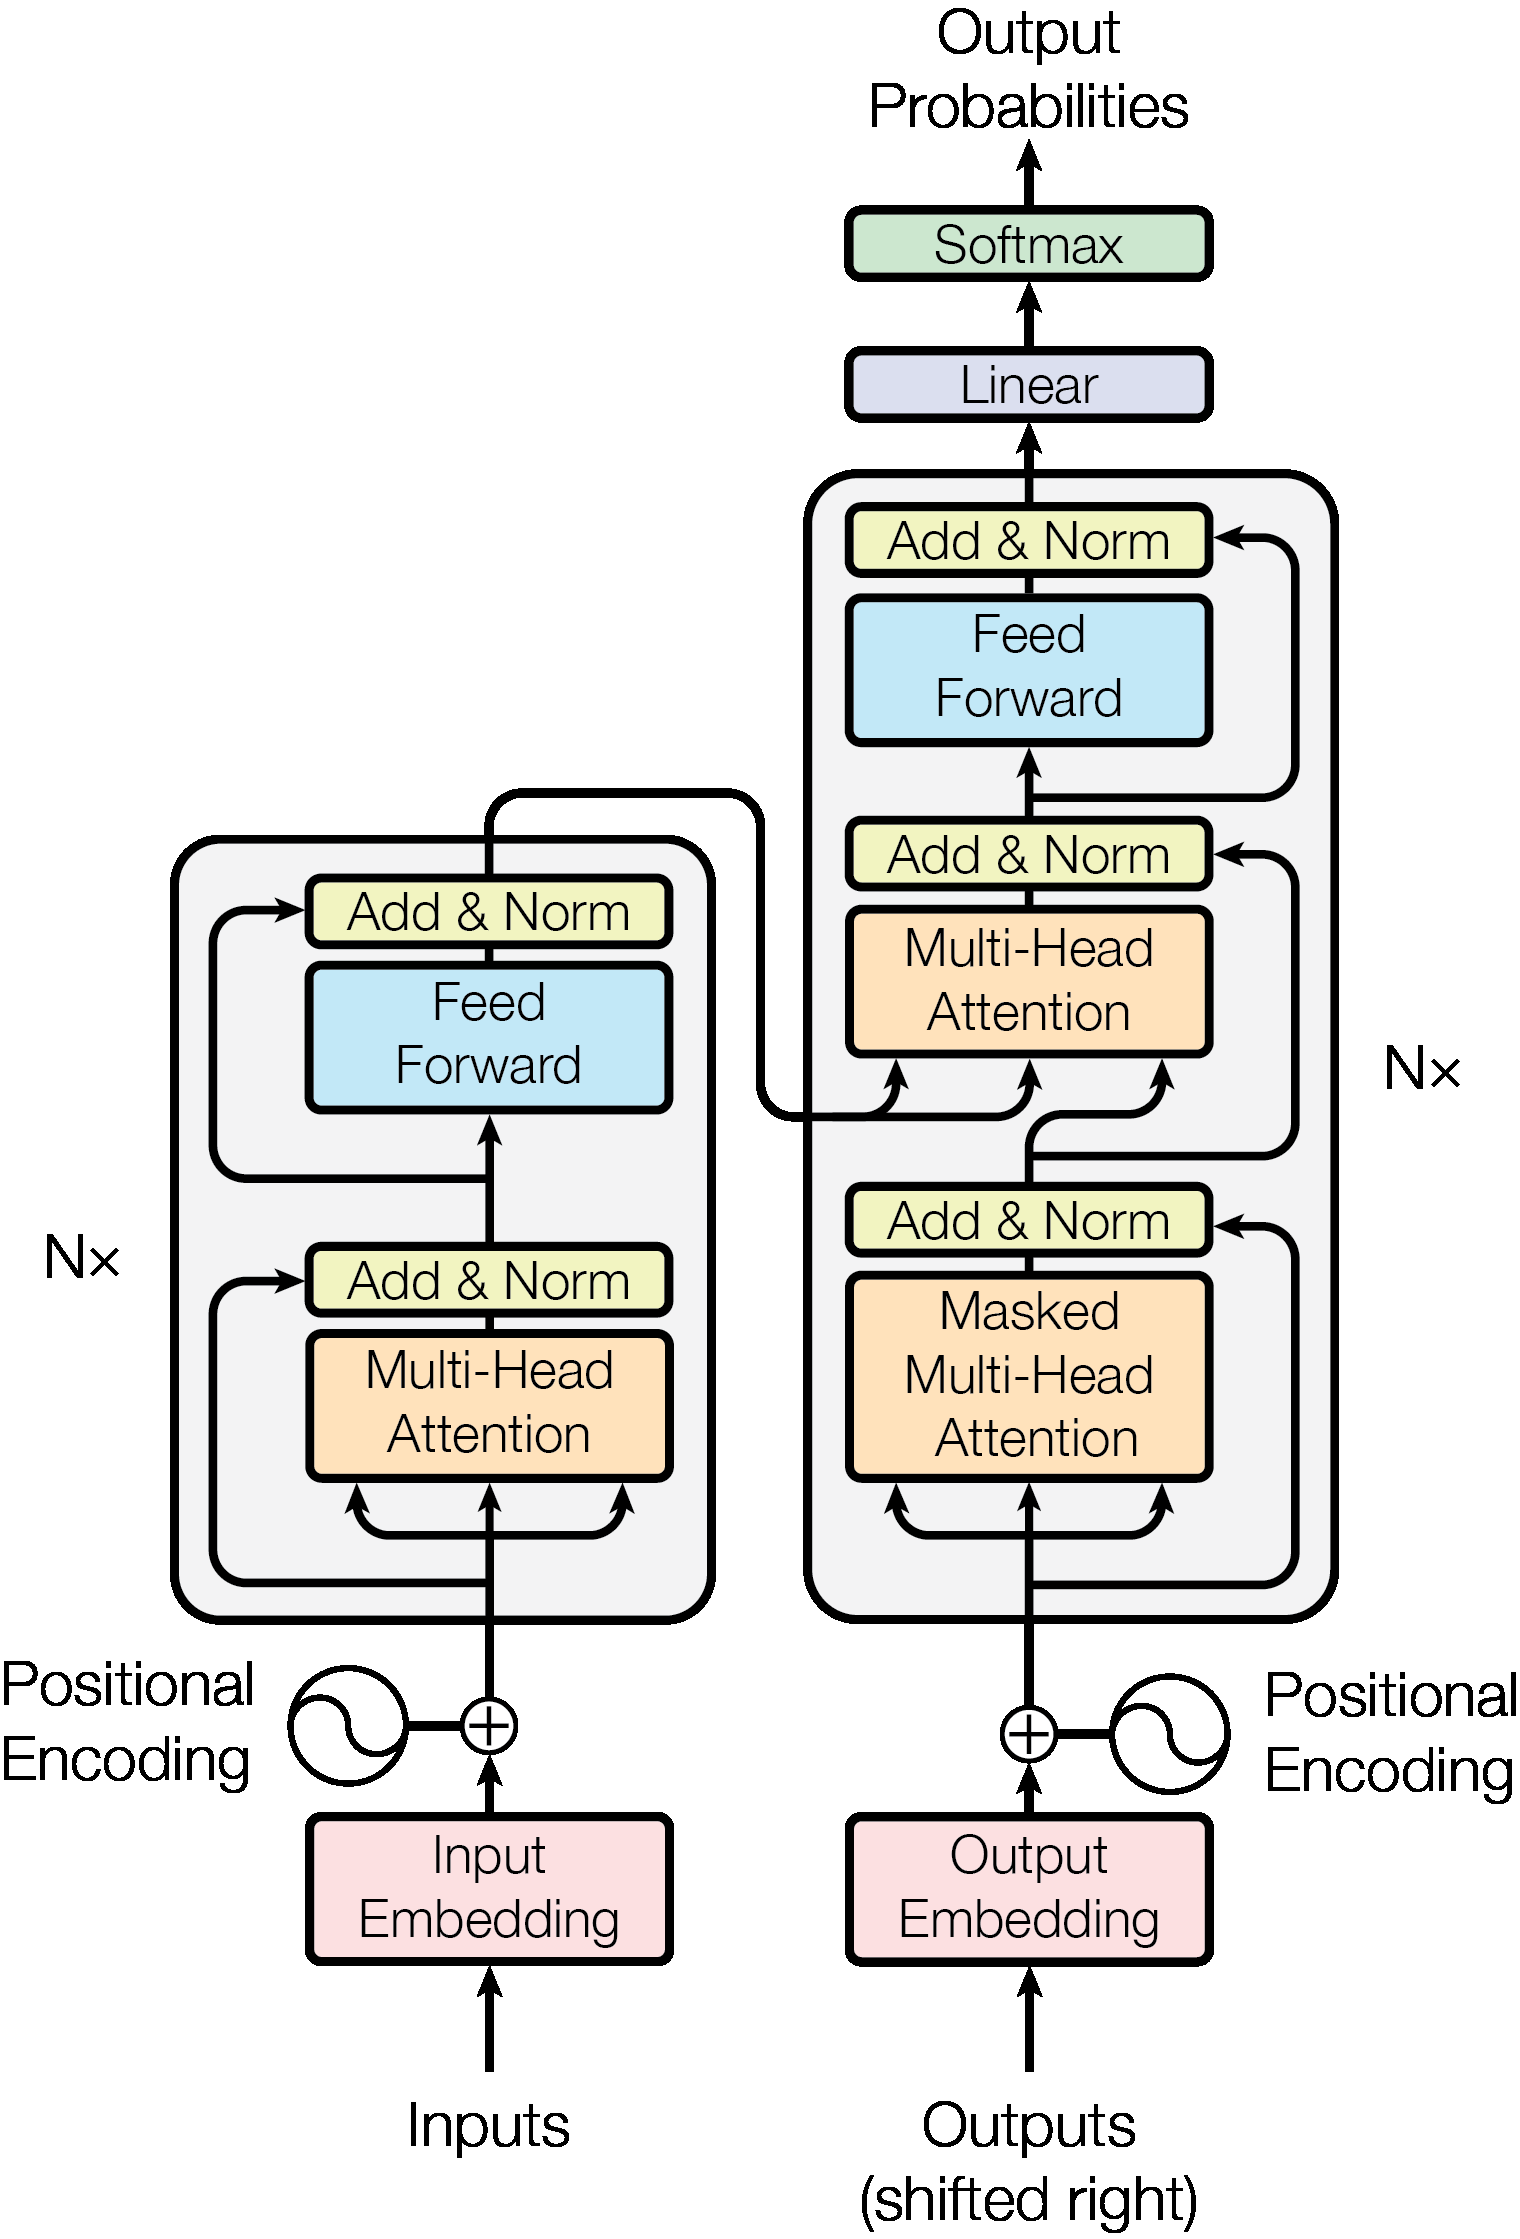
\includegraphics[width=\textwidth]{fig1_p3.png}

\vspace{2mm}
{\tiny The Transformer - model architecture.}

\end{column}
\end{columns}

\end{frame}


\begin{frame}{注意力机制 - Scaled Dot-Product Attention}

\begin{columns}[T]
\begin{column}{0.55\textwidth}

\begin{itemize}

    \item 输入：queries Q、keys K（维度dk）、values V（维度dv）

    \item 计算：Attention(Q,K,V) = softmax(QK\textasciicircum{}T/√dk)V

    \item 比加性注意力更快、更节省空间，可高度并行化

    \item 除以√dk防止点积过大导致softmax梯度消失

\end{itemize}

\end{column}
\begin{column}{0.42\textwidth}
\centering
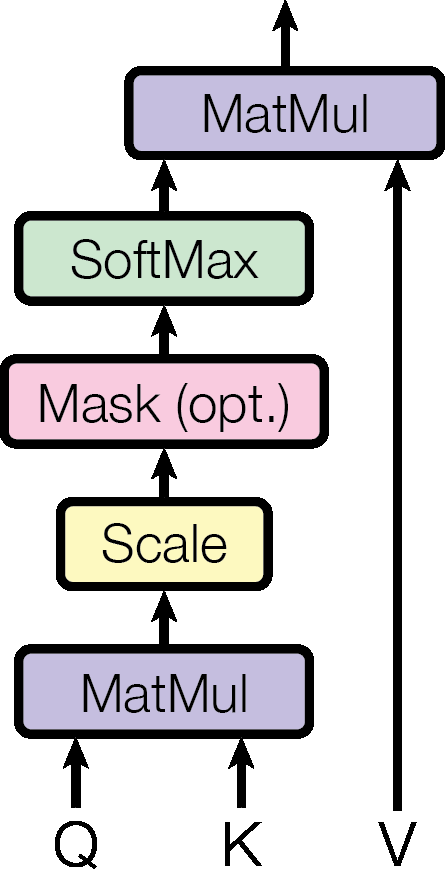
\includegraphics[width=\textwidth]{fig2_p4.png}

\vspace{2mm}
{\tiny Multi-head attention allows the model to jointly attend to information from diff}

\end{column}
\end{columns}

\end{frame}


\begin{frame}{注意力机制 - Multi-Head Attention}

\begin{columns}[T]
\begin{column}{0.55\textwidth}

\begin{itemize}

    \item 将Q、K、V投影h次到不同子空间（dk=dv=dmodel/h=64）

    \item MultiHead(Q,K,V) = Concat(head1,...,headh)W\textasciicircum{}O

    \item 允许模型同时关注不同表示子空间的信息

    \item 总计算成本与单头注意力相近，但效果显著提升

\end{itemize}

\end{column}
\begin{column}{0.42\textwidth}
\centering
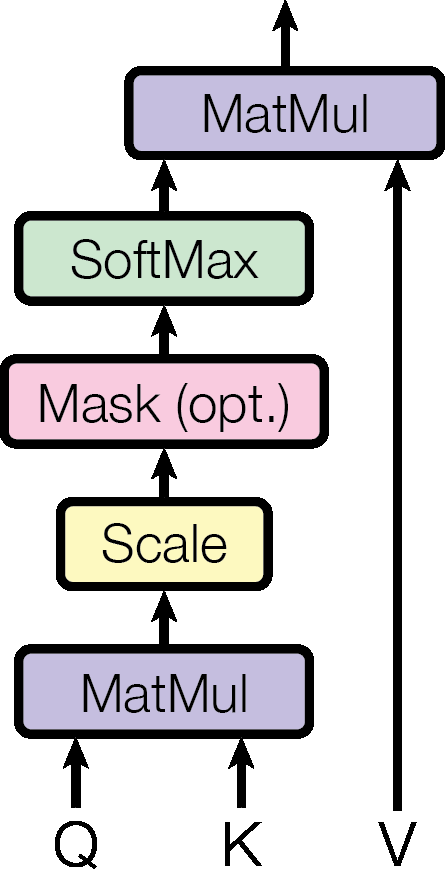
\includegraphics[width=\textwidth]{fig2_p4.png}

\vspace{2mm}
{\tiny Multi-head attention allows the model to jointly attend to information from diff}

\end{column}
\end{columns}

\end{frame}


\begin{frame}{位置编码与前馈网络}


\begin{itemize}

    \item 使用正弦/余弦函数生成位置编码，与嵌入向量相加

    \item PE(pos,2i) = sin(pos/10000\textasciicircum{}(2i/dmodel))

    \item 前馈网络：FFN(x) = max(0, xW1+b1)W2+b2

    \item 两层线性变换，内层维度dff=2048，激活函数ReLU

\end{itemize}


\end{frame}


\begin{frame}{机器翻译实验结果}


\begin{itemize}

    \item WMT 2014英德翻译：28.4 BLEU（最佳模型），超越所有集成模型2+ BLEU

    \item WMT 2014英法翻译：41.8 BLEU（新SOTA），训练仅需3.5天/8 GPU

    \item 比现有最佳模型的训练成本低数倍

    \item 基础模型：100K步训练12小时；大模型：300K步训练3.5天

\end{itemize}


\end{frame}


\begin{frame}{性能对比分析}


\begin{itemize}

    \item 英德翻译：Transformer(big) 28.4 vs 之前最佳26.3 (GNMT+RL Ensemble)

    \item 英法翻译：Transformer(big) 41.8 vs 之前最佳41.29 (ConvS2S Ensemble)

    \item 训练FLOPs显著降低：英德2.3×10\textasciicircum{}19 vs GNMT的1.4×10\textasciicircum{}20

    \item 验证了Transformer的高效性和优越性

\end{itemize}


\end{frame}


\begin{frame}{注意力可视化分析}

\begin{columns}[T]
\begin{column}{0.55\textwidth}

\begin{itemize}

    \item 注意力头能学习捕捉长距离依赖关系

    \item 图3：编码器第5层注意力准确关联'making'与'more difficult'

    \item 图4：部分注意力头专门处理回指解析（如'the Law'与'its application'）

    \item 证明模型学习到了句子的句法和语义结构

\end{itemize}

\end{column}
\begin{column}{0.42\textwidth}
\centering
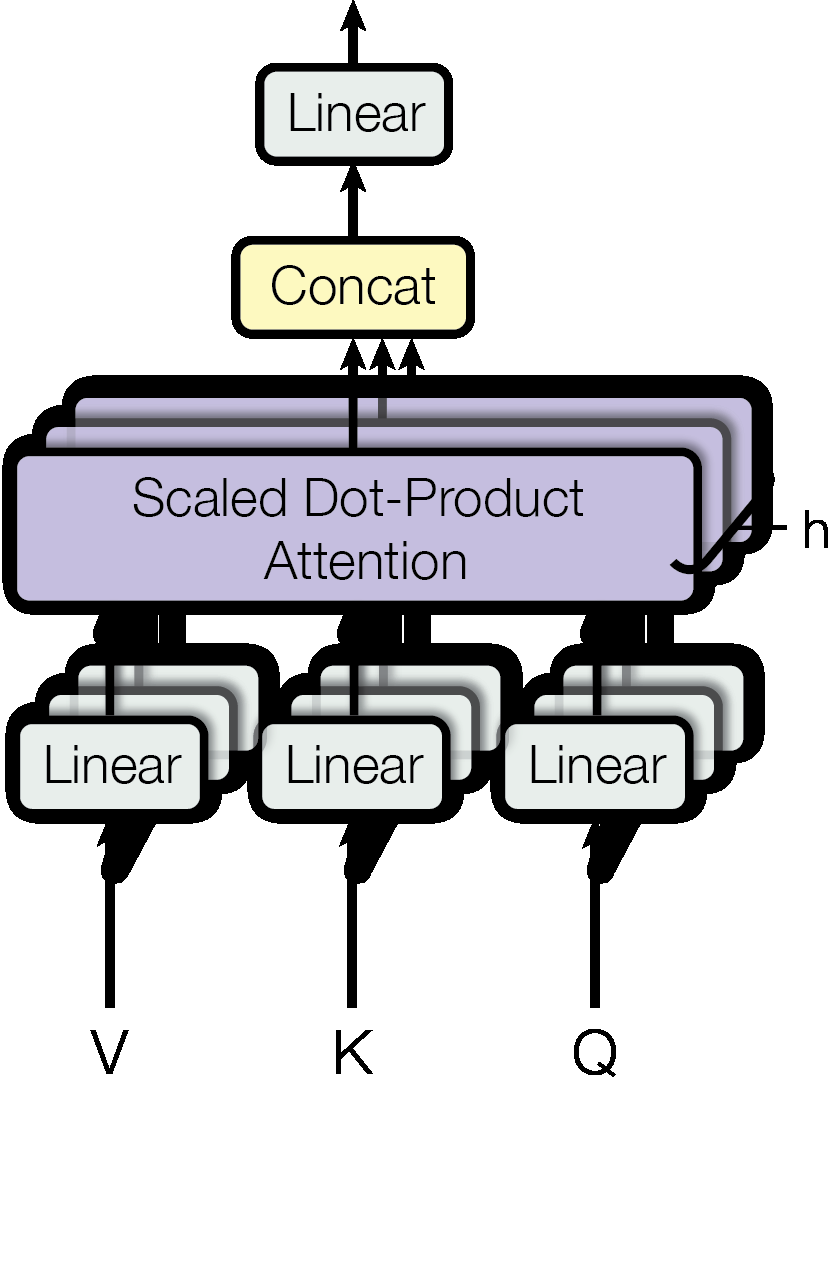
\includegraphics[width=\textwidth]{fig3_p4.png}

\vspace{2mm}
{\tiny An example of the attention mechanism following long-distance dependencies in th}

\end{column}
\end{columns}

\end{frame}


\begin{frame}{模型变体与消融实验}


\begin{itemize}

    \item (A) 头数和维度：8头、dk=dv=64为最佳，单头或多头过多均下降

    \item (B) 键维度：减小dk会损害模型质量，点积兼容性函数不可简化

    \item (C) 层数和大模型：大模型明显更优（dmodel=1024, dff=4096）

    \item (D) Dropout：Pdrop=0.1有效防止过拟合；(E) 位置编码：正弦与学习版效果相当

\end{itemize}


\end{frame}


\begin{frame}{泛化能力：成分句法分析}


\begin{itemize}

    \item 在英语成分句法分析任务上验证Transformer的泛化能力

    \item WSJ only设置：4层Transformer达到91.3 F1，超越BerkeleyParser

    \item 半监督设置（17M句子）：92.7 F1，接近最佳RNN Grammar模型

    \item 证明模型无需任务特定调优即可很好地迁移到其他NLP任务

\end{itemize}


\end{frame}


\begin{frame}{总结与展望}


\begin{itemize}

    \item Transformer是完全基于注意力机制的新架构，摒弃了RNN和卷积

    \item 在翻译任务上训练更快、质量更好，达到新的SOTA

    \item 证明了纯注意力模型的有效性和巨大潜力

    \item 未来方向：扩展到图像/音频/视频等模态，研究局部受限注意力

\end{itemize}


\end{frame}


\begin{frame}{参考文献}


\begin{itemize}

    \item [2] Bahdanau et al. Neural machine translation by jointly learning to align and translate. CoRR, 2014

    \item [9] Gehring et al. Convolutional sequence to sequence learning. arXiv, 2017

    \item [13] Hochreiter \& Schmidhuber. Long short-term memory. Neural computation, 1997

    \item [35] Sutskever et al. Sequence to sequence learning with neural networks. NIPS, 2014

    \item [38] Wu et al. Google's neural machine translation system. arXiv, 2016

\end{itemize}


\end{frame}



\end{document}